\documentclass[
  shownotes,
  xcolor={svgnames},
  hyperref={colorlinks,citecolor=DarkBlue,linkcolor=DarkRed,urlcolor=DarkBlue}
  , aspectratio=169]{beamer}
\usepackage{animate}
\usepackage{amsmath}
\usepackage{amsfonts}
\usepackage{amssymb}
\usepackage{pifont}
\usepackage{mathpazo}
%\usepackage{xcolor}
\usepackage{multimedia}
\usepackage{fancybox}
\usepackage[para]{threeparttable}
\usepackage{multirow}
\setcounter{MaxMatrixCols}{30}
\usepackage{subcaption}
\usepackage{graphicx}
\usepackage{lscape}
\usepackage[compatibility=false,font=small]{caption}
\usepackage{booktabs}
\usepackage{ragged2e}
\usepackage{chronosys}
\usepackage{appendixnumberbeamer}
\usepackage{animate}
\setbeamertemplate{caption}[numbered]
\usepackage{color}
%\usepackage{times}
\usepackage{tikz}
\usepackage{comment} %to comment
%% BibTeX settings
\usepackage{natbib}
\bibliographystyle{apalike}
\bibpunct{(}{)}{,}{a}{,}{,}
\setbeamertemplate{bibliography item}{[\theenumiv]}

% Defines columns for bespoke tables
\usepackage{array}
\newcolumntype{L}[1]{>{\raggedright\let\newline\\\arraybackslash\hspace{0pt}}m{#1}}
\newcolumntype{C}[1]{>{\centering\let\newline\\\arraybackslash\hspace{0pt}}m{#1}}
\newcolumntype{R}[1]{>{\raggedleft\let\newline\\\arraybackslash\hspace{0pt}}m{#1}}


\usepackage{xfrac}


\usepackage{multicol}
\setlength{\columnsep}{0.5cm}

% Theme and colors
\usetheme{Boadilla}

% I use steel blue and a custom color palette. This defines it.
\definecolor{andesred}{HTML}{af2433}

% Other options
\providecommand{\U}[1]{\protect\rule{.1in}{.1in}}
\usefonttheme{serif}
\setbeamertemplate{itemize items}[default]
\setbeamertemplate{enumerate items}[square]
\setbeamertemplate{section in toc}[circle]

\makeatletter

\definecolor{mybackground}{HTML}{82CAFA}
\definecolor{myforeground}{HTML}{0000A0}

\setbeamercolor{normal text}{fg=black,bg=white}
\setbeamercolor{alerted text}{fg=red}
\setbeamercolor{example text}{fg=black}

\setbeamercolor{background canvas}{fg=myforeground, bg=white}
\setbeamercolor{background}{fg=myforeground, bg=mybackground}

\setbeamercolor{palette primary}{fg=black, bg=gray!30!white}
\setbeamercolor{palette secondary}{fg=black, bg=gray!20!white}
\setbeamercolor{palette tertiary}{fg=white, bg=andesred}

\setbeamercolor{frametitle}{fg=andesred}
\setbeamercolor{title}{fg=andesred}
\setbeamercolor{block title}{fg=andesred}
\setbeamercolor{itemize item}{fg=andesred}
\setbeamercolor{itemize subitem}{fg=andesred}
\setbeamercolor{itemize subsubitem}{fg=andesred}
\setbeamercolor{enumerate item}{fg=andesred}
\setbeamercolor{item projected}{bg=gray!30!white,fg=andesred}
\setbeamercolor{enumerate subitem}{fg=andesred}
\setbeamercolor{section number projected}{bg=gray!30!white,fg=andesred}
\setbeamercolor{section in toc}{fg=andesred}
\setbeamercolor{caption name}{fg=andesred}
\setbeamercolor{button}{bg=gray!30!white,fg=andesred}

\makeatother


%%%%%%%%%%%%%%% BEGINS DOCUMENT %%%%%%%%%%%%%%%%%%

\begin{document}

\title[Lecture 2]{Lecture 2: \\ The classic and the predictive paradigms \\ Decision Theory}
\subtitle{Big Data and Machine Learning for Applied Economics \\ Econ 4676}
\date{\today}

\author[Sarmiento-Barbieri]{Ignacio Sarmiento-Barbieri}
\institute[Uniandes]{Universidad de los Andes}


\begin{frame}[noframenumbering]
\maketitle
\end{frame}

%%%%%%%%%%%%%%%%%%%%%%%%%%%%%%%%%%%
%       Motivation              %
% What is the question?
% Why do we care?
% What is new?
% What do you find?
%%%%%%%%%%%%%%%%%%%%%%%%%%%%%%%%%%%




\begin{frame}
\frametitle{Agenda}

\tableofcontents


\end{frame}



%%----------------------------------------------------------------------%

\section{Review}
\begin{frame}
\frametitle{Review}


{\bf Motivation}

\bigskip

\begin{itemize}
      \item We discussed the examples of Google Flu and Facebook face detection
      \medskip
      \begin{itemize}
        \item Take away, the success was driven by an empiric approach
        \item Given data  estimate a function $f(x)$ that predicts $y$ from $x$
      \end{itemize}
      \medskip

      \item  This is basically what we do as economists everyday so:
      \begin{itemize}
        \item  Are these algorithms merely applying standard techniques to novel and large datasets?
        \item  If there are fundamentally new empirical tools, how do they fit with what we know?
        \item  As empirical economists, how can we use them?
       \end{itemize}
\end{itemize}

\end{frame}
%----------------------------------------------------------------------%
\section{Shifting Paradigms}
\begin{frame}
\frametitle{Big vs Small, Classic vs Predictive}

\begin{itemize}
  \item Classical Stats (small data?)
    \begin{itemize}
      \item Get the most of few data (Gosset)
      \item Lots of structure, e.g. $X_1,X_2,...,X_n\sim t_v$
      \item Carefully curated $\rightarrow$ approximates random sampling (expensive, slow) but very good and reliable
    \end{itemize}
\bigskip
    \item Big Data (the 4 V's) 
    \begin{itemize}
      \item Data {\bf V}olume
      \item Data {\bf V}ariety
      \item Data {\bf V}elocity
      \item Data {\bf V}alue
      
    \end{itemize}

\end{itemize}
\bigskip



\end{frame}
%----------------------------------------------------------------------%
\begin{frame}
\frametitle{The Classic Paradigm}


\begin{align}
Y=f(X)+u
\end{align}
\medskip
\begin{itemize}
  \item Interest lies on inference
  \medskip
  \item "Correct" $f()$ to understand how Y is affected by X
  \medskip
  \item Model: Theory, experiment
  \medskip
  \item Hypothesis testing (std. err., tests)
\end{itemize}

\end{frame}

%----------------------------------------------------------------------%

\begin{frame}
\frametitle{The Predictive Paradigm}


\begin{align}
Y=f(X)+u
\end{align}

\begin{itemize}
  \item Interest on predicting $Y$
  \medskip
  \item "Correct" $f()$ to be able to predict (no inference!)
  \medskip
  \item Model?

\end{itemize}


\end{frame}


%----------------------------------------------------------------------%

\begin{frame}
\frametitle{How to choose $f(.)$}




\begin{figure}[H] \centering
  \centering
  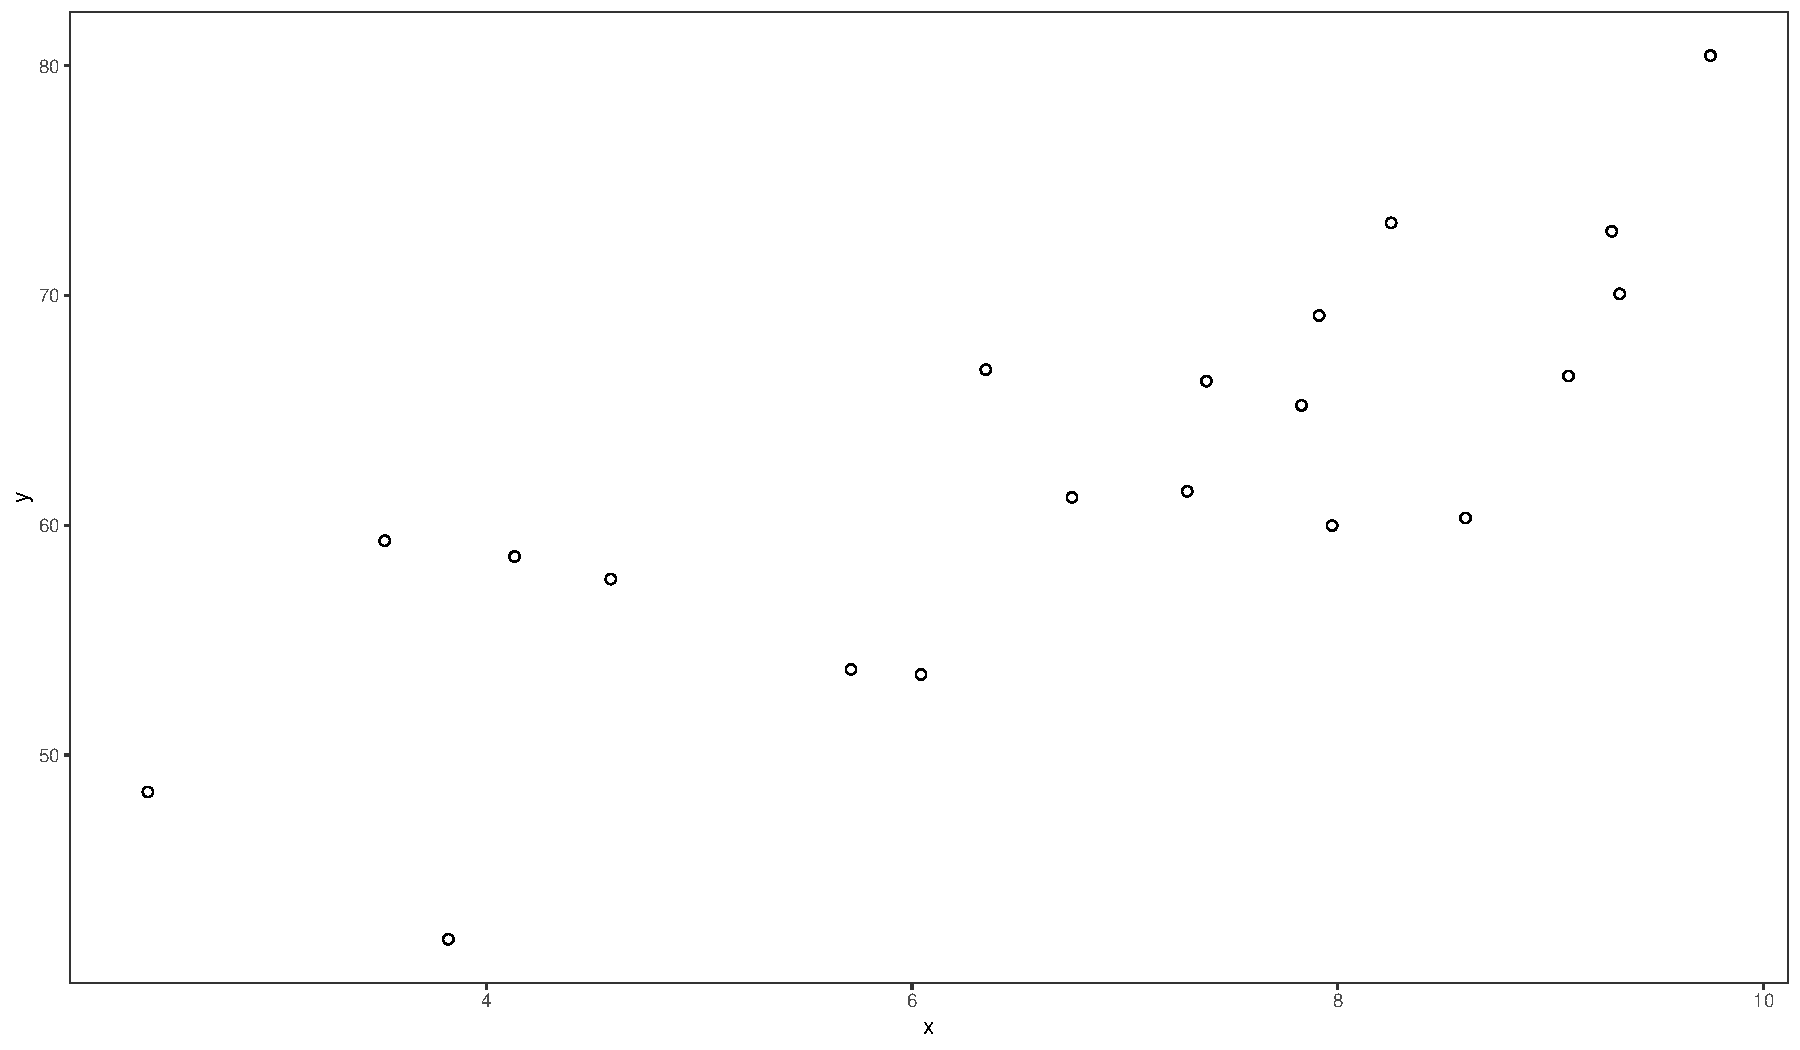
\includegraphics[scale=0.25]{figures/fig_1.pdf}
  \\
  \tiny
  Source: simulated data, see \texttt{figures} folder for scripts
\end{figure}


\end{frame}

%----------------------------------------------------------------------%

\begin{frame}
\frametitle{How to choose $f(.)$}


\begin{itemize}
  \item Linear $f(X)=X\beta$
\end{itemize}

\begin{figure}[H] \centering
  \centering
  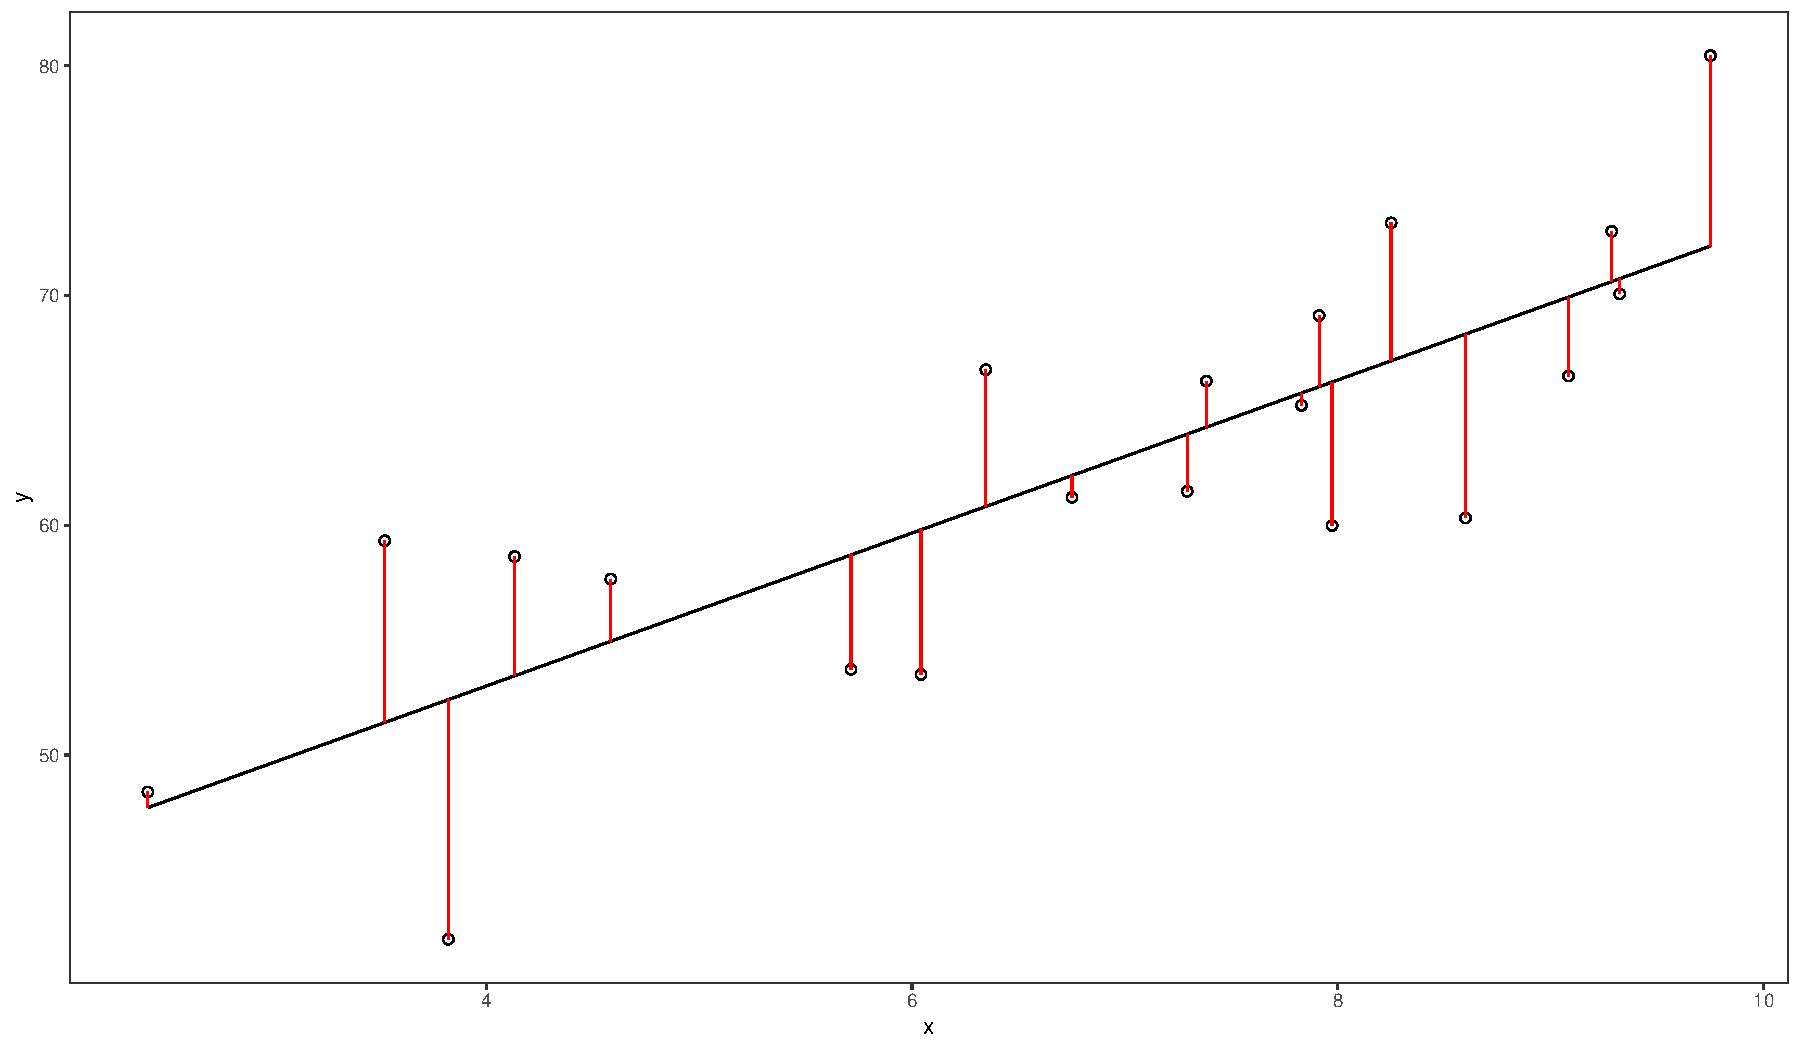
\includegraphics[scale=0.25]{figures/fig_1b.pdf}
  \\
  \tiny
  Source: simulated data, see \texttt{figures} folder for scripts
\end{figure}


\end{frame}
%----------------------------------------------------------------------%

\begin{frame}
\frametitle{How to choose $f(.)$}


\begin{itemize}
  \item Spline $f(X)=g(X)$, where g is a spline
\end{itemize}

\begin{figure}[H] \centering
  \centering
  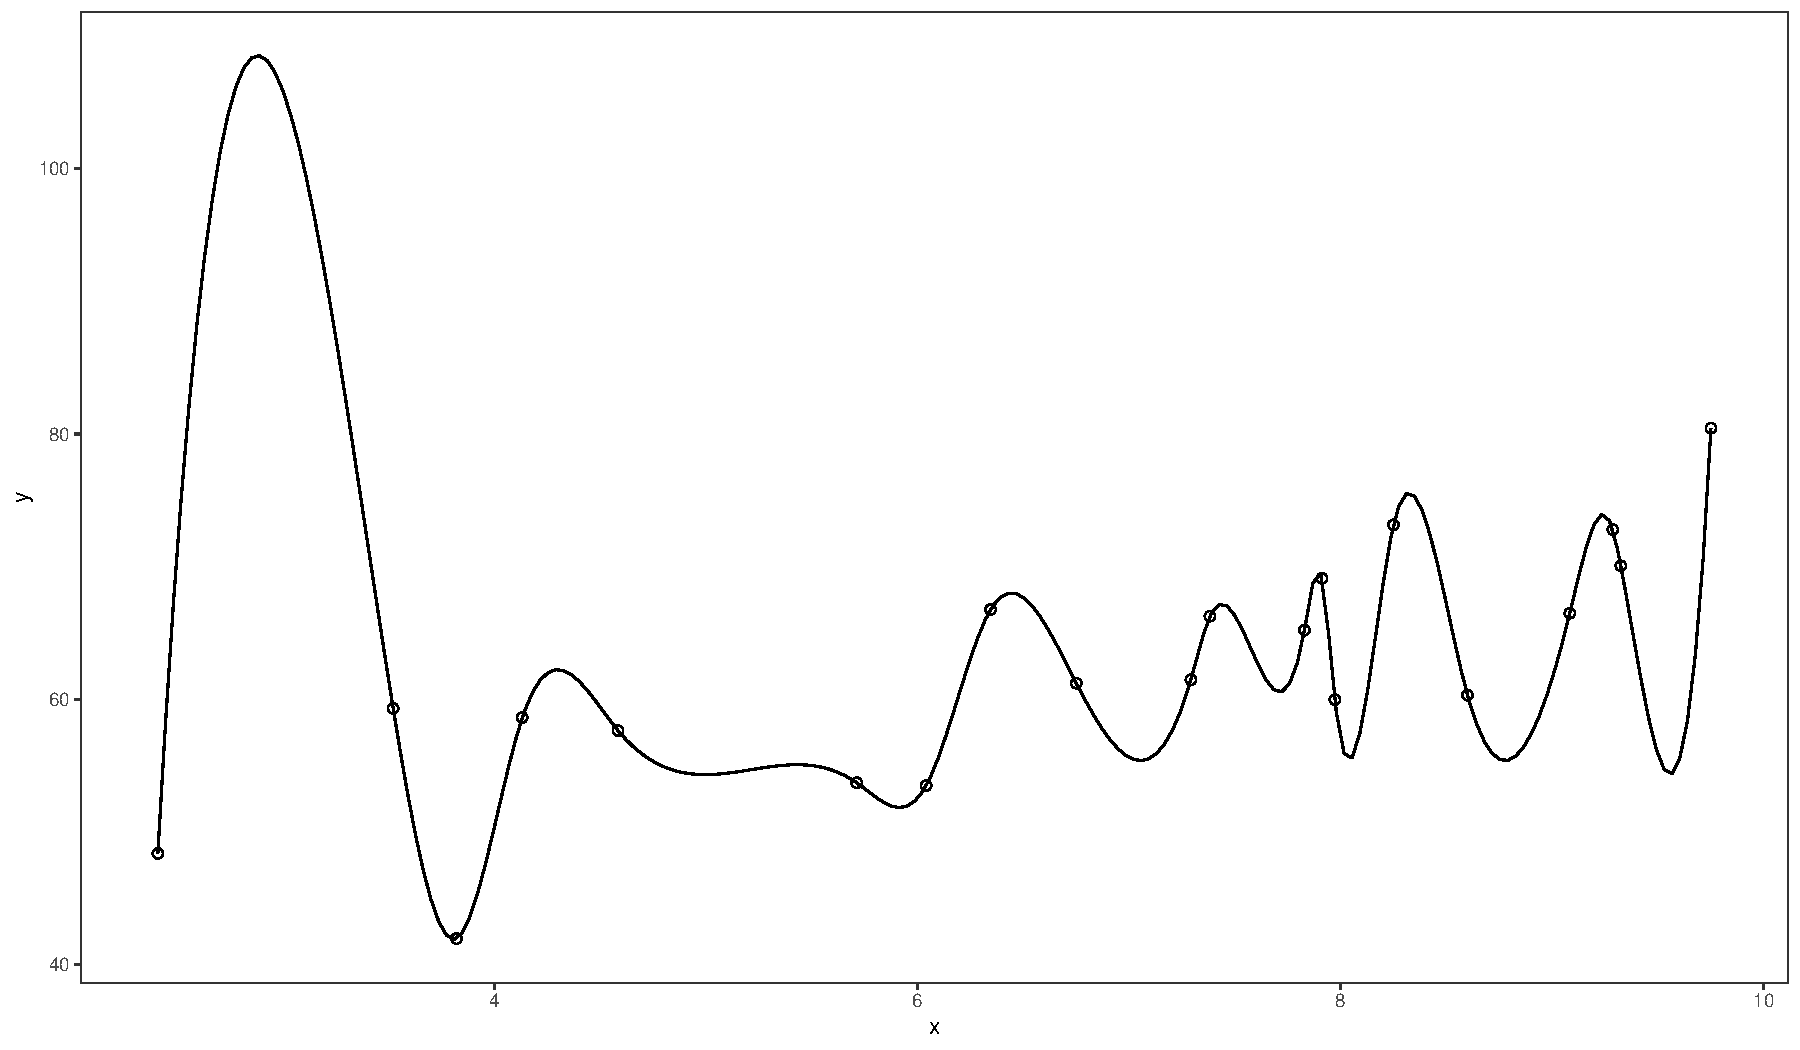
\includegraphics[scale=0.25]{figures/fig_1c.pdf}
  \\
  \tiny
  Source: simulated data, see \texttt{figures} folder for scripts
\end{figure}
\end{frame}







%----------------------------------------------------------------------%
\section{How to Evaluate Estimators?}
%----------------------------------------------------------------------%
\section{Statistical Decision Theory}
\begin{frame}
\frametitle{Statistical Decision Theory: A bit of theory}

\begin{itemize}
  \item We need a bit of theory to give us a framework for choosing $f$
  \item A decision theory approach involves an {\bf action space} $\mathcal{A}$
  \item The {\bf action space} $\mathcal{A}$ specify the possible "actions we might take"
  \item Some examples
\end{itemize}

\footnotesize

\begin{table}[H]
\caption{Action Spaces}

\begin{centering}
\begin{tabular}{cc}
\hline
Inference & Action Space\\
\hline
\hline
Estimation $\theta$, $g\left(\theta\right)$  & $\mathcal{A}=\Theta$\\
Prediction & $\mathcal{A}=space\,of\,X_{n+1}$\\
Model Selection & $\mathcal{A}=\left\{ Model\,I,Model\,II,...\right\} $\\
Hyp. Testing & $\mathcal{A}=\left\{ Reject|Accept\,H_{0}\right\} $\\

\hline
\end{tabular}
\par\end{centering}
\end{table}


\end{frame}

%----------------------------------------------------------------------%

\begin{frame}
\frametitle{Statistical Decision Theory: A bit of theory}


\begin{itemize}
  \item After the data $X=x$ is observed, where $X\sim f(X|\theta)$, $\theta \in \Theta$
  \item A decision is made
  \item The set of allowable decisions is the action space ($\mathcal{A}$)
  \item The loss function in an estimation problem reflects the fact that if an action $a$ is close to $\theta$,
  \begin{itemize}
   \item then the decision $a$ is reasonable and little loss is incurred.
   \item if it is far then a large loss is incurred
  \end{itemize}
\end{itemize}

\begin{align}
    L:\mathcal{A}\rightarrow\left[0,\infty\right]
\end{align}


\end{frame}
%----------------------------------------------------------------------%

\begin{frame}
\frametitle{Statistical Decision Theory: A bit of theory}
\framesubtitle{Loss Function}

\begin{itemize}
\item If $\theta$ is real valued, two of the most common loss functions are

\begin{itemize}
  \item Squared Error Loss:

  \begin{align}
      L(a,\theta)=(a-\theta)^{2}
  \end{align}

    \item Absolute Error Loss:

    \begin{align}
      L(a,\theta)=|a-\theta|
    \end{align}
\end{itemize}


\item These two are symmetric functions. However, there's no restriction. For example in hypothesis testing a "0-1" Loss is common.
\item Loss is minimum if the action is correct
\end{itemize}
%how $L$ looks as longs as it maps into $\left[0,\infty\right]$.
\end{frame}
%----------------------------------------------------------------------%

\begin{frame}
\frametitle{Statistical Decision Theory: A bit of theory}
\framesubtitle{Risk Function}
In a decision theoretic analysis, the quality of an estimator is quantified by its risk function, that is, for an estimator $\delta(x)$ of $\theta$, the risk function is

\begin{align}
      R(\theta,\delta)=E_\theta (L(\theta,\delta(X))
    \end{align}

    at a given $\theta$, the risk function is the average loss that will be incurred if the estimator $\delta(X)$ is used


\begin{itemize}
\item Since $\theta$ is unknown we would like to use an estimator that has a small value of $R(\theta,\delta)$ for all values $\theta$
\item Loss is minimum if the action is correct
\item If we need to compare two estimators ($\delta_1$ and $\delta_2$) then we will compare their risk functions
\item If $R(\delta_1,\theta)<R(\delta_2,\theta)$ for all $\theta \in \Theta$, then $\delta_1$ is preferred because it performs better for all $\theta$

\end{itemize}
\end{frame}
%----------------------------------------------------------------------%

\begin{frame}
\frametitle{Statistical Decision Theory: A bit of theory}
\framesubtitle{Example: Binomial Risk Function}

\begin{itemize}
  \footnotesize
  \item Let $X_1,X_2,...X_n \sim Bernoulli(p)$
  \item Consider 2 estimators for $p$:  $\hat{p}^1=\frac{1}{n}\sum X_i$ and $\hat{p}^2=\frac{\sum X_i + \sqrt{n/4}}{n+\sqrt{n}}$
  \item Their risks are: $R(\hat{p}^1,p)=\frac{p(1-p)}{n}$ and $R(\hat{p}^2,p)=\frac{n}{4(n+\sqrt{n})^2}$
\end{itemize}


\begin{figure}
\centering
\begin{subfigure}{.5\textwidth}
  \centering
  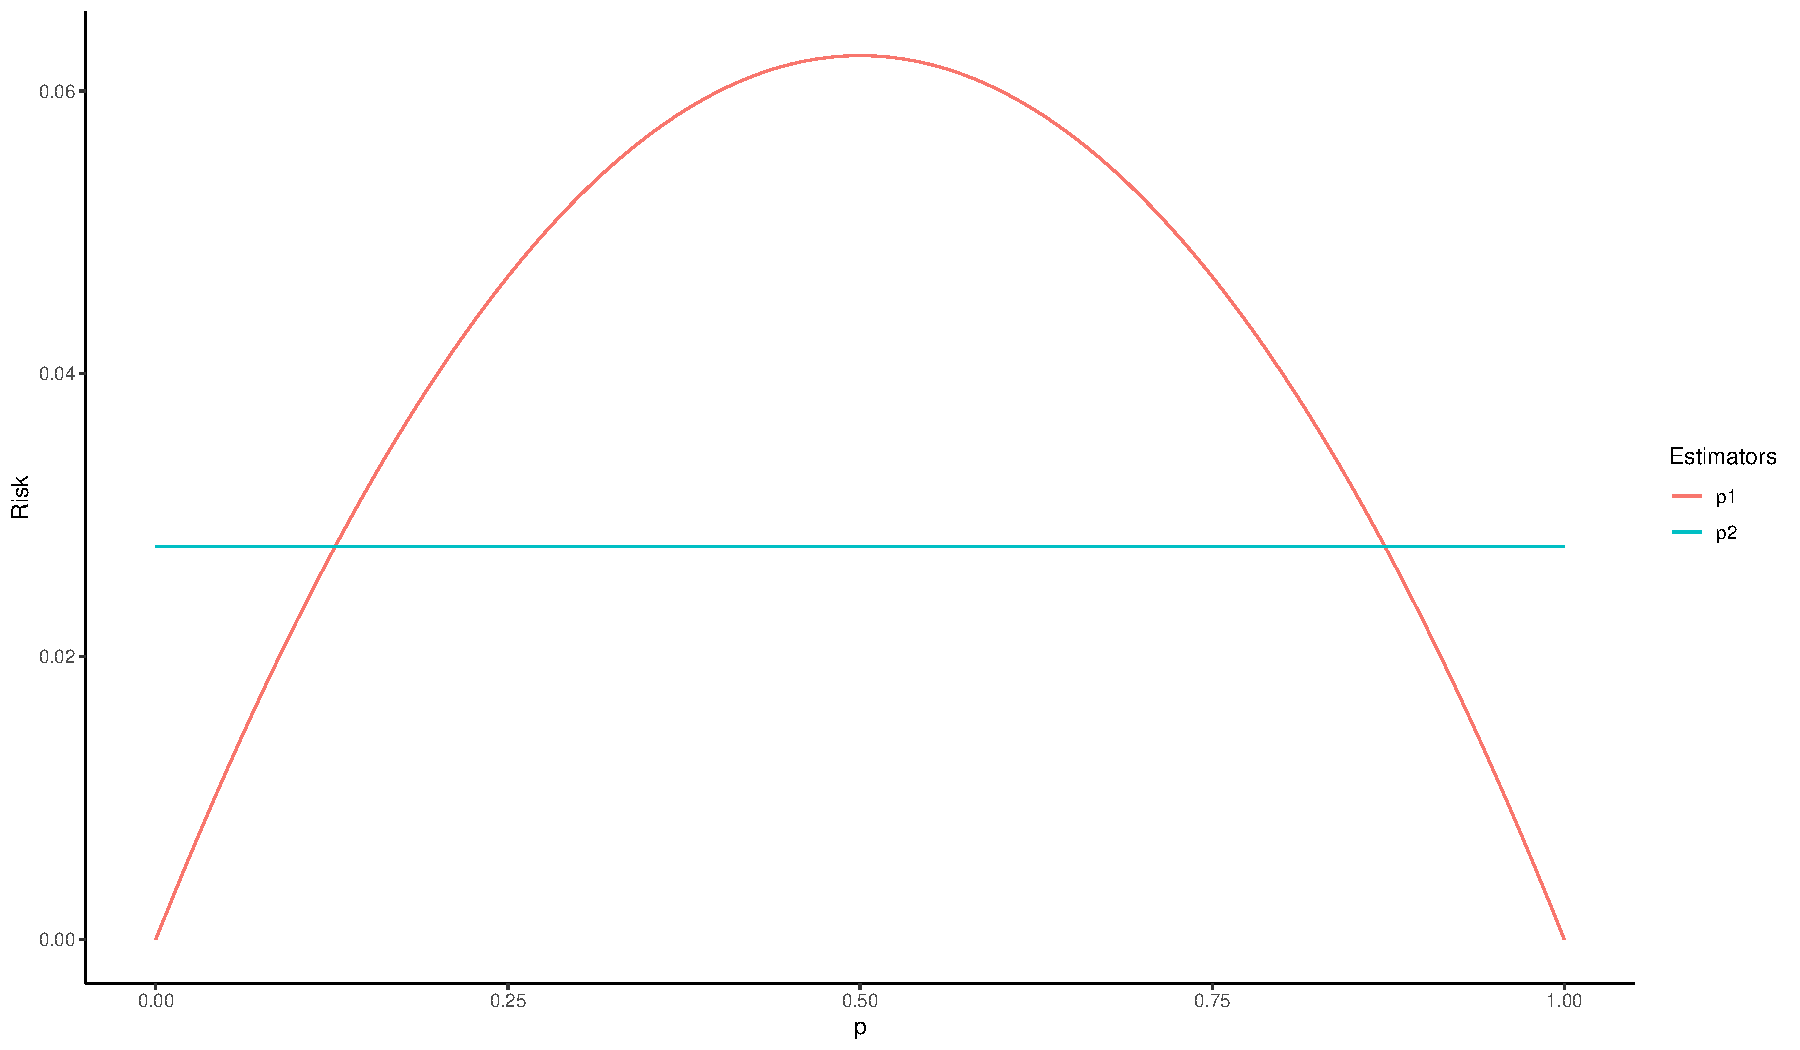
\includegraphics[scale=0.23]{figures/fig_2a.pdf}
  \caption{n=4}
\end{subfigure}%
\begin{subfigure}{.5\textwidth}
  \centering
  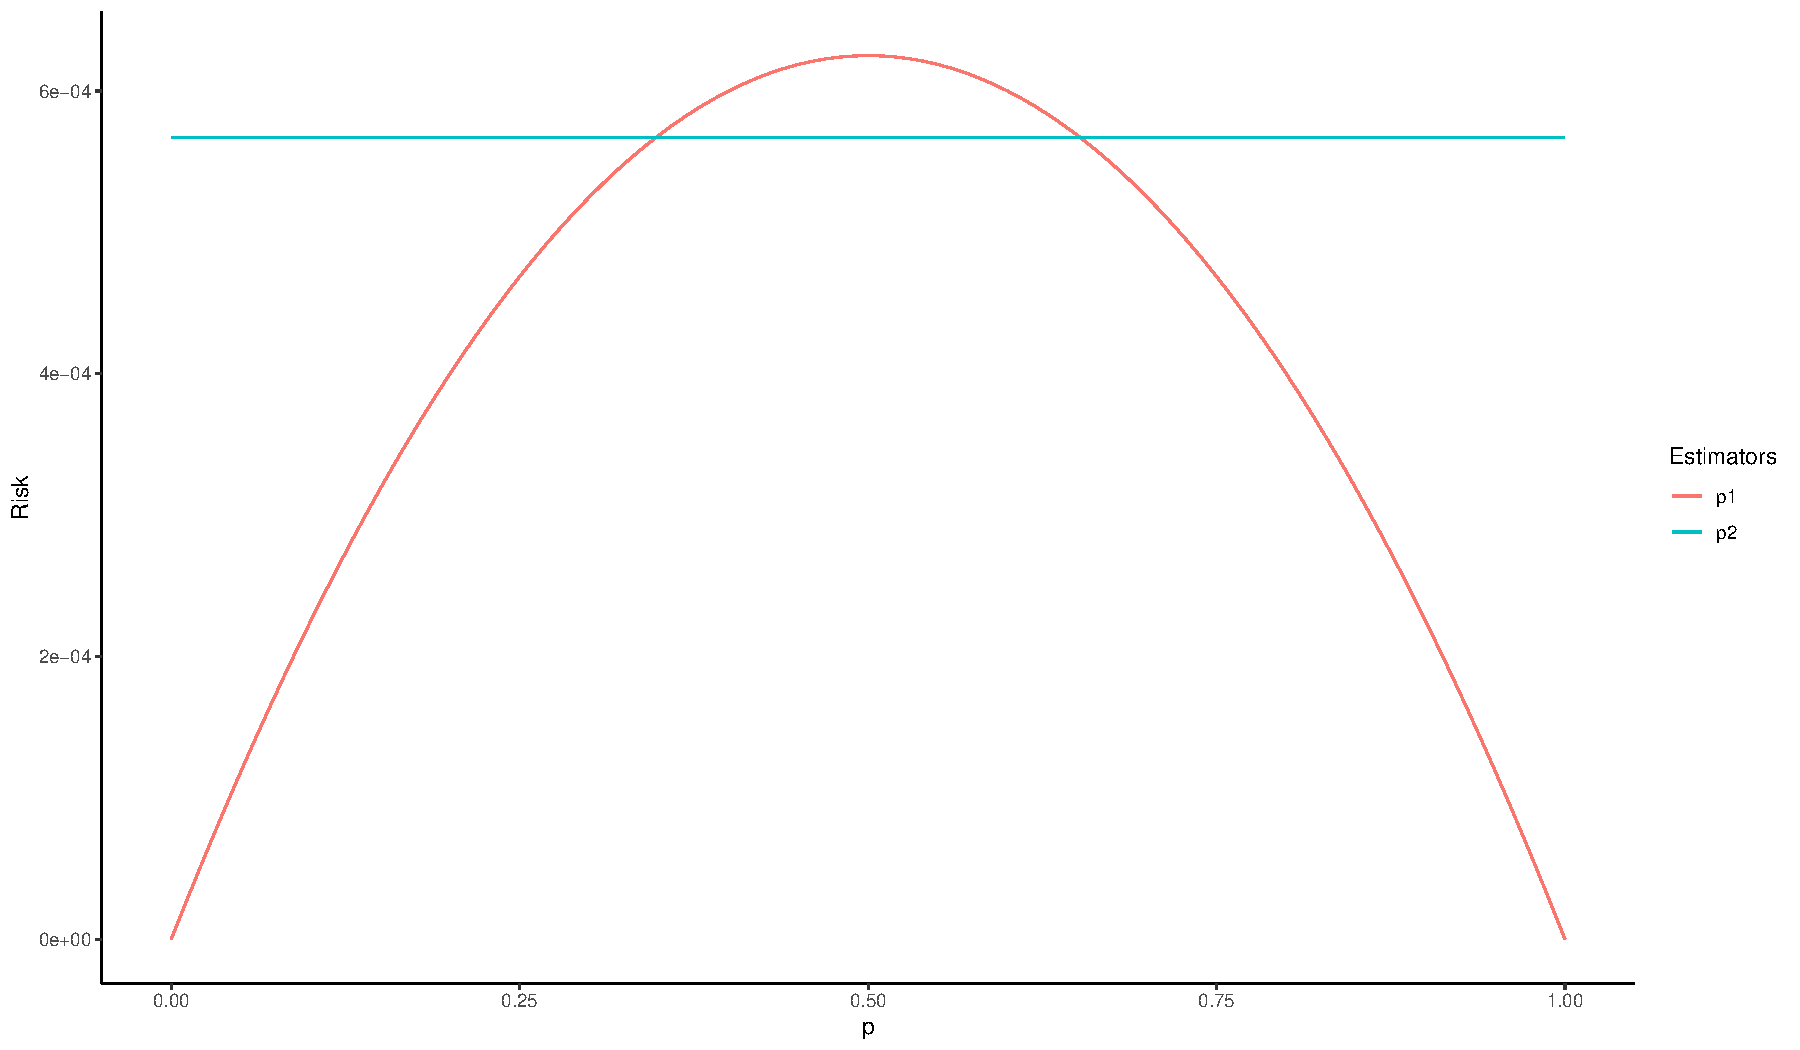
\includegraphics[scale=0.23]{figures/fig_2b.pdf}
  \caption{n=400}
\end{subfigure}
\end{figure}



\end{frame}
%----------------------------------------------------------------------%

\begin{comment}
\begin{frame}
\frametitle{Statistical Decision Theory: A bit of theory}
\framesubtitle{Risk Function}

\textbf{Frequentist Approach}

\[
E_{\theta}L\left(\delta\left(\underline{X}\right),\theta\right)=R\left(\delta,\theta\right)
\]

note that $\underline{X}$ are generated from a model with parameter
$\theta$.

\textbf{Bayesian Approach}

\[
E_{\theta}\left[L\left(\delta\left(\underline{X}\right),\theta\right)|\theta=\theta_{0}\right]=R\left(\delta,\theta_{0}\right)
\]

In the bayesian approach the data is generated from $\underline{X}|\theta=\theta_{0}$,
the parameter is not fixed, comes from a distribution.

\end{frame}
\end{comment}
%----------------------------------------------------------------------%
\begin{frame}

\frametitle{ Decision Theory for prediction}
\framesubtitle{How to choose f?}
\begin{itemize}
  \item In a prediction problem we want to predict $Y$ from $f(X)$ in such a way that the loss is minimum
  \item Assume also that $X \in \mathbb{R}^p$ and $Y \in \mathbb{R}$ with joint distribution $Pr(X,Y)$
\end{itemize}

\begin{align}
  R(Y,f(X)) &=E[(Y-f(X))^2] \\
            &=\int (y-f(x))^2 Pr(dx,dy)
\end{align}

conditioning on X we have that
\begin{align}
 R(Y,f(X)|X) &= E_X E_{Y|X} [(Y-f(X))^2|X]
\end{align}

this risk is also known as the {\bf mean squared (prediction) error} $MSE(f)$ 
\end{frame}
%----------------------------------------------------------------------%

\begin{frame}
\frametitle{ Decision Theory for prediction}


It suffices to minimize  the $MSE(f)$ point wise so

\begin{align}
f(x)= argmin_m E_{Y|X} [(Y-m)^2|X=x)
\end{align}

Y a random variable and m a constant (predictor)

\begin{align}
min_m E(Y-m)^2= \int (y-m)^2  f(y)dy
\end{align}
\medskip
{\bf Result}: The best prediction of $Y$ at any point $X = x$ is the conditional mean, when best is measured using a square error loss

\end{frame}
%----------------------------------------------------------------------%

\begin{frame}[t]
\frametitle{ Decision Theory for prediction}

{\bf Proof} \\
\medskip
FOC
\medskip
\begin{align}
\int -2 (y-m)  f(y)  dy =0
\end{align}
\medskip
Dividing by -2 and reorganizing
\medskip
\begin{align}
 m \int f(y) dy = \int y f(y)  dy
\end{align}


\end{frame}
%----------------------------------------------------------------------%

\begin{frame}
\frametitle{ Decision Theory for prediction}


\begin{align}
 m \int (y) dy = \int y f(y)  dy
\end{align}
\begin{align}
m=E(Y|X=x)
\end{align}


The best prediction of $Y$ at any point $X = x$ is the conditional expectation function (CEF), when best is measured using a square error loss
\begin{itemize}
\item What shape does the CEF take?
\item Linear 
\begin{itemize}
\item $(y,X)$ are jointly normal
\item When models are saturated.
\end{itemize}
\end{itemize}


\end{frame}
%----------------------------------------------------------------------%

\begin{frame}
\frametitle{Linear Regression}

\begin{itemize}
\item Note the following from the {\it Regression-CEF Theorem}

The function $X'\beta$ provides the minimum risk  linear approximation to $E(Y|X)$, that is

\begin{align}
\beta = \underset{b}{argmin}\,E\left\{ (E(Y|X) - X'b)^2 \right\}
\end{align}

\item Proof 
\begin{align}
(Y - X'b)^2 &= {(Y- E(Y|X))+ (E(Y|X) - X'b)}^2 \\
            &= (Y- E(Y|X))^2+ (E(Y|X) - X'b)^2 + 2 (Y- E(Y|X))(E(Y|X) - X'b)
\end{align}

\item The CEF approximation problem then has the same solution as the population least square problems

%\item this is why it is so important for us

\end{itemize}
\end{frame}

%----------------------------------------------------------------------%
\section{Linear Regression}
%----------------------------------------------------------------------%
\begin{frame}
\frametitle{Linear Regression}

\begin{itemize}


  \item Regression provides the best linear predictor for the dependent variable in the same way that the CEF is the best unrestricted predictor of the dependent variable. 
  \medskip
  

  \item The fact that Regression approximates the CEF is useful because it helps describe the essential features of statistical relationships, without necessarily trying to pin them down exactly. 
  \medskip

  \item Linear regression is the “work horse” of econometrics and (supervised) machine learning. 
  \medskip
  \item Very powerful in many contexts.
  \medskip
  \item Big `payday' to study this model in detail.
\end{itemize}
\end{frame}


%----------------------------------------------------------------------%
\begin{frame}
\frametitle{Linear Regression Model}
\bigskip
$f(X)=X\beta$, estimating $f(.)$ boils down to estimating $\beta$
\begin{align}
y = X \beta +u
\end{align}

where 
\begin{itemize}
  \item y is a vector $n \times 1$ with typical element $y_i$
  \item X is a matrix $n \times k$ 
  \begin{itemize}
    \tiny
      \item Note that we can represent it as a column vector $\underset{n\times k}{X}=[\underset{n\times 1}{X_1}\,\,\underset{n\times 1}{X_2}\dots \underset{n\times 1}{X_k}] $
  \end{itemize}
  \item $\beta$ is a vector $k \times 1$ with typical element $\beta_j$
\end{itemize}

\bigskip
Thus 

\begin{align}
y_i &= X_i' \beta +u_i  \\ \nonumber
    &= \sum_{j=1}^k \beta_j X_{ji} +u_i
\end{align}

\end{frame}

%----------------------------------------------------------------------%
\begin{frame}
\frametitle{Linear Regression Model}

How do we estimate $\beta$?

\begin{itemize}
  \footnotesize
  \item Method of Moments {\tiny (for HW)}
  \item MLE {\tiny (more on this later)}
  \item OLS: minimize risk squared error loss $\rightarrow$ minimizes SSR ($e'e$) 
  \begin{itemize}
    \tiny
  \item where $e=Y-\hat Y=Y-X\hat\beta$
  \item In the HW, you will show that min SSR same as max $R^2$
  \end{itemize}  
\end{itemize}
\bigskip

OLS solution: $\hat \beta = (X'X)^{-1} X'y$

\bigskip
\begin{figure}[H] \centering
  \centering
  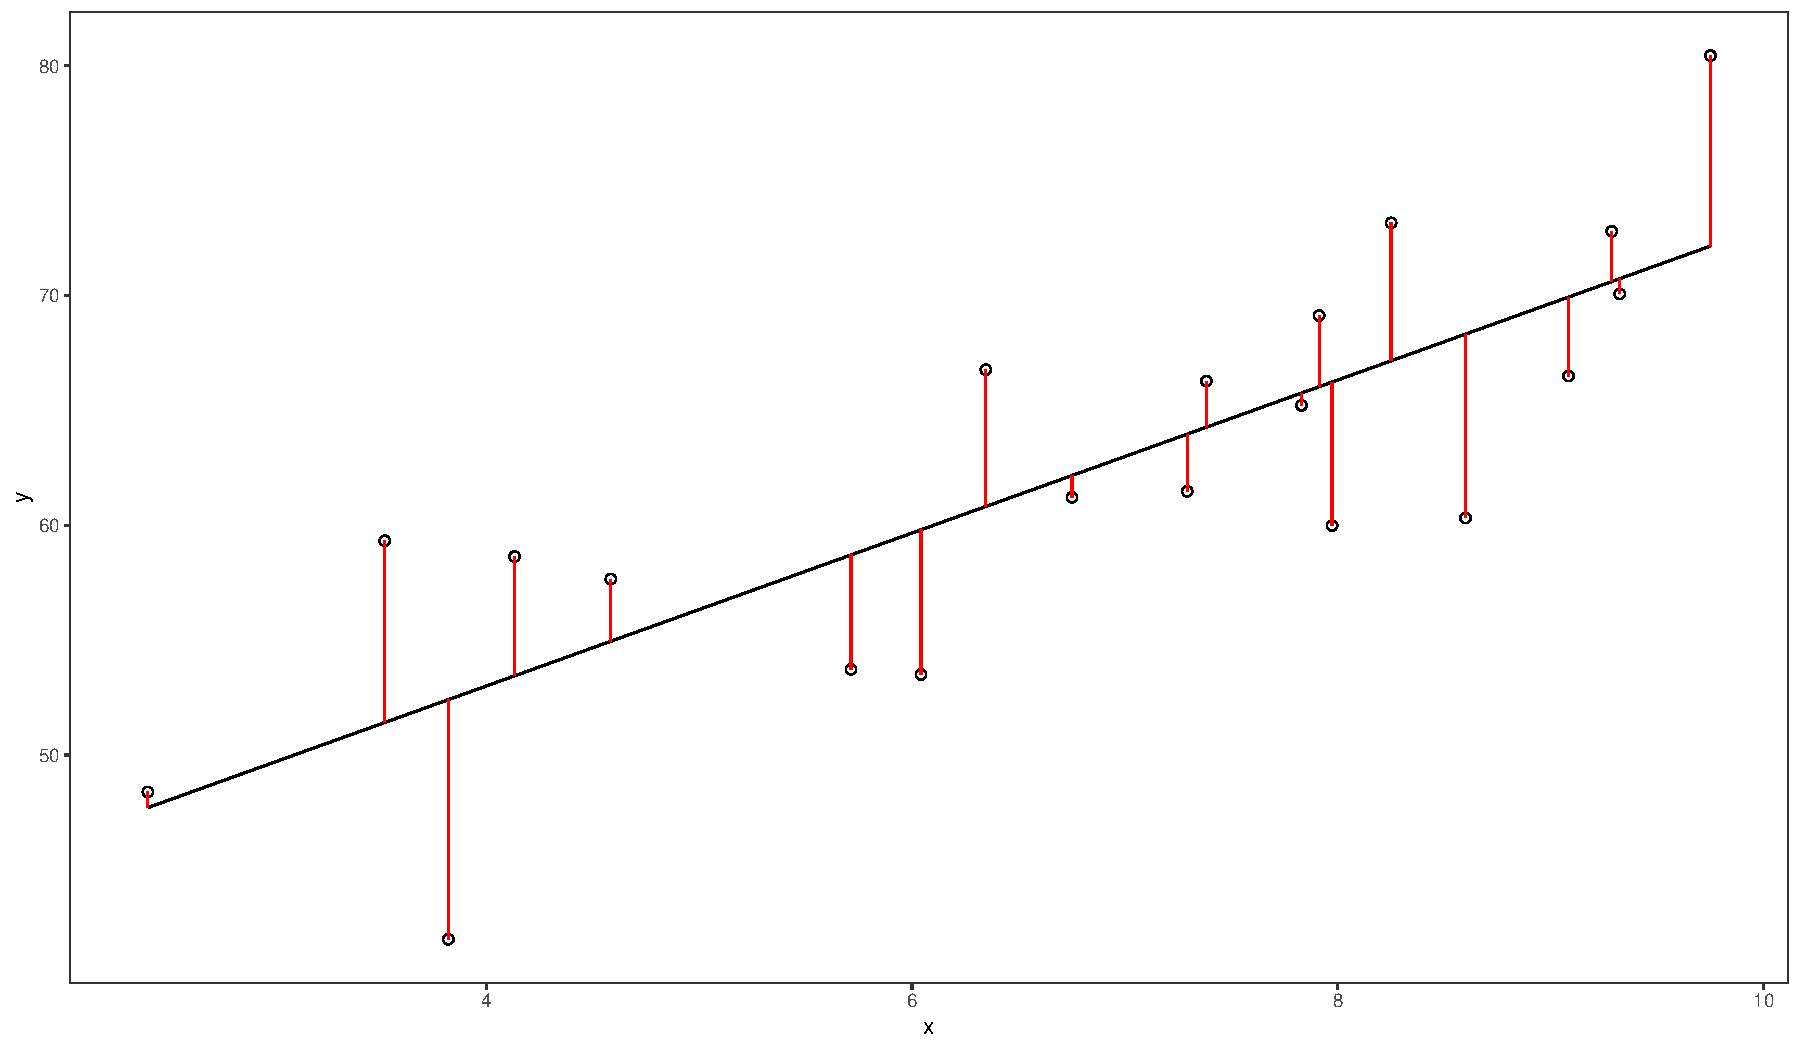
\includegraphics[scale=0.22]{figures/fig_1b.pdf}
  \\
  \tiny
\end{figure}


\end{frame}
%----------------------------------------------------------------------%
\begin{frame}
\frametitle{Gauss Markov Theorem}


Gauss-Markov Theorem says that 
\bigskip
\begin{align}
 \hat \beta = (X'X)^{-1} X'y
\end{align}

\bigskip

\begin{itemize}
  \item The OLS estimator ($\hat \beta$) is BLUE, the more efficient than any other linear unbiased estimator, 
  \medskip
  \item Efficiency in the sense that  $Var(\tilde \beta) - Var(\hat \beta)$ is positive semidefinite matrix.
\end{itemize}

\bigskip
\tiny Proof: HW. Tip: a matrix $M_{p\times p}$ is positive semi-definite iff $c'Mc\geq0$ $\forall x\in \mathbb{R}^p$

\end{frame}


%----------------------------------------------------------------------%
\begin{frame}
\frametitle{Gauss Markov Theorem}

\begin{itemize}
  \item Gauss Markov Theorem that says OLS is BLUE is perhaps one of the most famous results in statistics. 
  
  \begin{itemize}
    \item $E(\hat\beta) = \beta$
    \medskip 
    \item $V(\hat \beta ) = \sigma^2 (X'X)^{-1}$
  \end{itemize}
  
\bigskip
  \item However, it is essential to note the limitations of the theorem. 

  \begin{itemize}
    \footnotesize
    \item Correctly specified with exogenous Xs, 
      \medskip 
    \item The term error is homoscedastic 
      \medskip 
    \item No serial correlation.
      \medskip 
    \item Nothing about the OLS estimator being the more efficient than any other estimator one can imagine.
  \end{itemize}
    
    %\medskip 
    %\item Estimators that are nonlinear and/or biased may have a better performance than OLS 
  

\end{itemize}

\end{frame}


%----------------------------------------------------------------------%
\begin{frame}
\frametitle{Prediction vs Estimation}

\begin{itemize}
\item {\bf Predicting well in this context $\rightarrow$ estimating well}

  \bigskip 
\begin{itemize}
  \item Note that the prediction of $y$ will be given by $\hat y=X \hat \beta$
  \bigskip 
  \item Under Gauss-Markov framework
  
  \begin{itemize}
    \item $E(\hat y) = X\beta$
    \medskip 
    \item $V(\hat y ) = \sigma^2 X' (X'X)^{-1} X$
  \end{itemize}
\end{itemize}

  \bigskip 

\item Then if $\hat \beta$ is unbiased and of minimum variance, 
\item then $\hat y$ is an unbiased predictor and minimum variance, from the class of unbiased linear estimators/predictors
  \begin{itemize}
    \tiny 
    \item Proof: for HW similar to $\hat \beta$ proof
  \end{itemize}
\end{itemize}
\end{frame}




%----------------------------------------------------------------------%
\section{Recap}
\begin{frame}
\frametitle{Recap}

\begin{itemize}
    \item We start shifting paradigms
    \medskip
    \item Tools are not that different (so far)
    \medskip
    \item Decision Theory: Risk with square error loss $\rightarrow$ MSE
    \medskip
    \item OLS is a "work horse" approximates the $E[Y|X]$ quite well 
    \medskip
    \item Next Class:
    \medskip
    \begin{itemize}
    \item  Next Class: OLS, Geometry, Properties
    \end{itemize}
     
\end{itemize}
\end{frame}

%----------------------------------------------------------------------%

\begin{frame}
\frametitle{Further Readings}

\begin{itemize}
  \item Angrist, J. D., \& Pischke, J. S. (2008). Mostly harmless econometrics. Princeton university press.
  \bigskip
  \item Casella, G., \& Berger, R. L. (2002). Statistical inference (Vol. 2, pp. 337-472). Pacific Grove, CA: Duxbury.
  \bigskip 
  \item Tom Shaffer The 42 V’s of Big Data and Data Science. \url{https://www.kdnuggets.com/2017/04/42-vs-big-data-data-science.html}
\end{itemize}

\end{frame}

%----------------------------------------------------------------------%
\end{document}
%----------------------------------------------------------------------%


